


 \documentclass[12t]{article}
 
 \usepackage[margin=1in]{geometry} 
 \usepackage{amsmath,amsthm,amssymb, mathtools}
 \usepackage{graphicx}
 \usepackage{subcaption}
 \usepackage{wrapfig}
 \usepackage{natbib}
 \bibliographystyle{plain}
 
 % Used to create code windows for Java
 \usepackage{listings}
 \usepackage{color}
 
 \definecolor{dkgreen}{rgb}{0,0.6,0}
 \definecolor{gray}{rgb}{0.5,0.5,0.5}
 \definecolor{mauve}{rgb}{0.58,0,0.82}
 
 \lstset{frame=tb,
 	language=Java,
 	aboveskip=3mm,
 	belowskip=3mm,
 	showstringspaces=false,
 	columns=flexible,
 	basicstyle={\small\ttfamily},
 	numbers=none,
 	numberstyle=\tiny\color{gray},
 	keywordstyle=\color{blue},
 	commentstyle=\color{dkgreen},
 	stringstyle=\color{mauve},
 	breaklines=true,
 	breakatwhitespace=true,
 	tabsize=3
 }

  
  \begin{document}
 	% PUT YOUR TITLE AND NAME HERE
 	\newcommand{\titlestr}{Mining Big Data - Map-Reduce}
 	\newcommand{\shorttitlestr}{Assignment 3}
 	\newcommand{\groupnames}{Matthew Vincent}
 	\newcommand{\studentids}{a1148120}
 	\newcommand{\authorstr}{\groupnames}
 	
 	%%%%%%%%%%%%%%%%%%%%%%%%%%%%%%555
 	% title page
 	\begin{titlepage}
 		\centering
 		
 		{\LARGE \bf \titlestr \par}
 		\vspace{0.25cm}
 		{\large \bf \shorttitlestr \par}
 		
 		
 		\vspace{1cm}
 		{\large \authorstr \\}
 		{ \studentids \par}
 		\vspace{0.25cm}
 		
 		\large School of Computer Science, The University of Adelaide
 		
 		\vspace{1cm}
 		\today
 		
 		\vspace{3cm}
 		Report submitted for
 		{\bf COMP SCI 3306 Mining Big Data}
 		at the School of Computer Science,
 		University of Adelaide
 		
 		
\includegraphics[width=0.35\textwidth]{./Figures/UoA_logo_cmyk.pdf}
 		
 		\vspace{9cm}
 		

 	 	\vspace{1mm}
 		\noindent \hrulefill
 		
 		\vfill
 	\end{titlepage}
 	
 	\clearpage
 	\setcounter{page}{1}
	
	\section*{Exercise 1}

	

	\newpage
	
	\section*{Exercise 2}

	\subsection*{Part 1}
	
	To perform a hierarchical clustering on the one-dimensional set of points provided, each iteration will be displayed below. An iteration begins with a set of clusters, each containing points to assigned to the cluster at previous iterations. The centroid for each cluster is also displayed. 	
	
	Pairs of clusters with the lowest distance between centroids are clustered together in the iteration. If there are an odd number of clusters at the beginning of the iteration, one cluster will remain that has not been assigned to a new cluster at that iteration.
	
	A dendrogram has been included to display the overall process of the hierarchical clustering, terminating once all points have been assigned to a single cluster. 
	
	\subsubsection*{Iteration 1}

	\begin{tabular}{ccc}
	Cluster & Member Points & Centroid \\
	\hline
  	1. & 1 & 1 \\
 	2. & 4 & 4 \\
 	3. & 9 & 9 \\
 	4. & 16 & 16 \\
 	5. & 25 & 25 \\
 	6. & 36 & 36 \\
 	7. & 49 & 49 \\
 	8. & 64 & 64 \\
  	9. & 81 & 81 \\
	\hline 
	\end{tabular} \\\\
	Resulting clusters after iteration 1: (1, 4), (9, 16), (25, 36), (49, 64), (81).
	
	\subsubsection*{Iteration 2}

	\begin{tabular}{ccc}
	Cluster & Member Points & Centroid \\
	\hline
  	1. & (1, 4) & 2.5 \\
 	2. & (9, 16) & 12.5 \\
 	3. & (25, 36) & 30.5 \\
 	4. & (49, 64) & 56.5 \\
 	5. & (81) & 81 \\
	\hline 
	\end{tabular} \\\\
	Resulting clusters after iteration 2: (1, 4, 9, 16), (25, 36), (49, 64, 81).
	
	\subsubsection*{Iteration 3}

	\begin{tabular}{ccc}
	Cluster & Member Points & Centroid \\
	\hline
  	1. & (1, 4, 9, 16) & 7.5 \\
 	2. & (25, 36) & 30.5 \\
 	3. & (49, 64, 81) & 64.67 \\
	\hline 
	\end{tabular} \\\\
	Resulting clusters after iteration 3: (1, 4, 9, 16, 25, 36), (49, 64, 81).
	
	\subsubsection*{Iteration 4}

	\begin{tabular}{ccc}
	Cluster & Member Points & Centroid \\
	\hline
  	1. & (1, 4, 9, 16, 25, 36) & 15.17 \\
 	2. & (49, 64, 81) & 64.67 \\
	\hline 
	\end{tabular} \\\\
	Resulting clusters after iteration 4: (1, 4, 9, 16, 25, 36, 49, 64, 81).	
	
	\begin{figure}[h]
	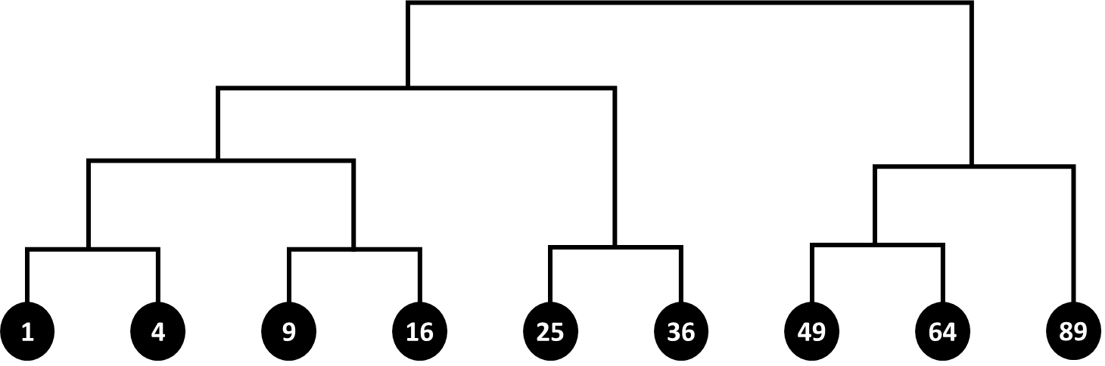
\includegraphics[width=0.8\textwidth]{./Figures/dendrogram.png}\\	
	\caption{Dendrogram illustrating hierarchical clustering of one-dimensional points}
	\end{figure}
	
	\newpage	
	
	\subsection*{Part 2}
	
	asdffasdf

	
	\section*{Exercise 3}
	
	\subsection*{Part 1}	
	
	To see that the greedy algorithm will assign at least 4 out of the 6 queries, consider a hypothetical worst case scenario where as few queries are assigned as possible. 
	
	Suppose we faced a worst case scenario where no queries are assigned. In this case, advertiser $A$ would obviously not be assigned any queries. The only way that this could happen is if $A$ was not assigned either of the first two queries, since $A$ only bids on $x$. Therefore, we can restrict our worst case to only those assignment combinations where either advertiser $B$ or advertiser $C$ bids on the first two queries. 
	
	Now, since $B$ and $C$ both bid on query $x$, we know that the first two queries will be assigned, regardless of whether $B$ or $C$ bids on the first of them. And since $B$ and $C$ both bid on $y$, we know that the third and fourth queries in the sequence will also be assigned, regardless of which advertiser is assigned the first two queries. 
	
	Hence, the greedy algorithm will necessarily assign at least 4 of the 6 queries. 

	\subsection*{Part 2}
	
	Consider the sequence of queries $xxzzzz$. The optimal algorithm would be able to assign 4 of these queries to an advertiser, for example, by assigning the first two to advertiser $A$ and the second two to advertiser $C$. However, since each advertiser only has a budget of 2, and since only $C$ bids on query $z$, the optimal algorithm will not be able to achieve more than 4 assignments in the sequence. 
	
	Now consider the greedy algorithm. The first two queries could be assigned to advertiser $C$, who bids on $x$, $y$, and $z$. Advertiser $C$'s budget would then be exhausted, with neither $A$ or $B$ bidding on the remaining queries. Hence, the greedy algorithm achieves 2 assignments compared to the optimal algorithm assigning 4, meaning that the greedy algorithm has only assigned half the queries of the optimal.

\bibliography{./bibliography-ChapterSummary}
\end{document}
